\section{Wertbestimmungs-Methode festlegen}
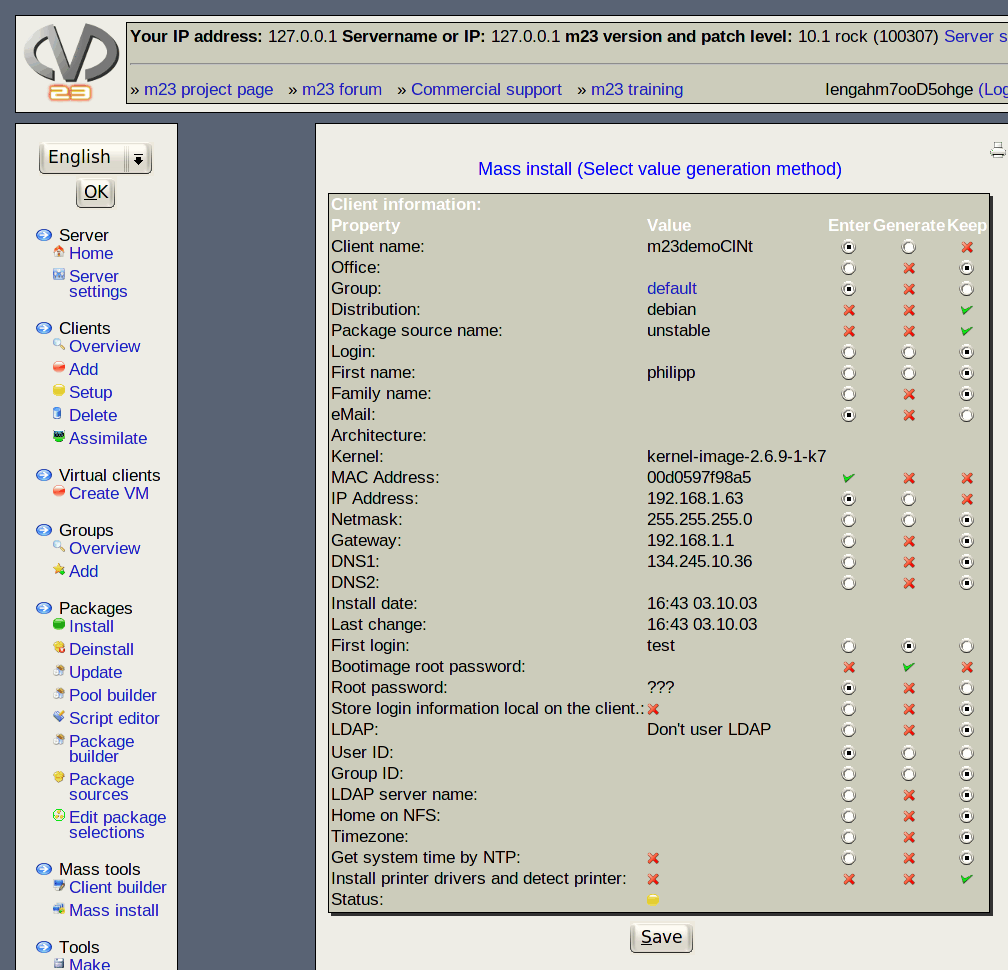
\includegraphics[scale=0.4]{/mdk/doc/manual/screenshots/de/mi_step0.png} \\
Hier k�nnen Sie festlegen, wie die Eigenschaftswerte der Clients generiert werden sollen.\\
\subsection{Es stehen 3 Methoden zur Auswahl}
\begin{itemize}
\item \textbf{Eingeben}: Die Eigenschaften werden per Hand eingegeben oder aus einer Datei eingelesen.\\
\item \textbf{Generieren}: Die Werte werden automatisch generiert. Z.B. k�nnen Clientnamen mit fortlaufenden Nummern erstellt oder freie IP-Adressen verwendet werden.\\
\item \textbf{Beibehalten}: Der im "definierten Client" festgelegte Wert wird f�r alle Clients beibehalten.\\
\end{itemize}
Bei einigen Eigenschaften ist nur eine eingeschr�nkte Auswahl m�glich, nicht w�hlbare Wertbestimmungs-Methoden sind durch ein rotes Kreuz gekennzeichnet. Ein gr�ner Haken bedeutet, da� dies die einzige m�gliche Methode f�r eine Eigenschaft ist. So kann eine MAC-Adresse weder generiert werden, noch f�r alle Clients gleich sein. Deshalb mu� sie per Hand eingegeben oder aus einer Datei eingelesen werden.\\
